\section{Geometric Foundations}

Feature-based face morphing requires us to deform one facial geometry so that landmarks align with those of another face.  The workhorse for this deformation is the \emph{piecewise affine warp}: we triangulate the landmark sets, then apply an affine transformation to each corresponding triangle pair.  In this section we build the full mathematical machinery --- affine transformations, barycentric coordinates, and inverse mapping --- that makes the warp both exact and hole-free.

%-----------------------------------------------------------------------
\subsection{Affine Transformations --- Theory}
%-----------------------------------------------------------------------

An \textbf{affine transformation} in 2D is a mapping
\[
    f : \mathbb{R}^2 \to \mathbb{R}^2,
    \qquad f(\mathbf{x}) = \mathbf{A}\,\mathbf{x} + \mathbf{t},
\]
where $\mathbf{A} \in \mathbb{R}^{2 \times 2}$ is a linear transformation matrix and $\mathbf{t} \in \mathbb{R}^2$ is a translation vector.  Written component-wise for a point $(x, y)$ mapped to $(x', y')$:
\[
\begin{bmatrix} x' \\ y' \end{bmatrix}
=
\begin{bmatrix}
    a_{11} & a_{12} \\
    a_{21} & a_{22}
\end{bmatrix}
\begin{bmatrix} x \\ y \end{bmatrix}
+
\begin{bmatrix} t_x \\ t_y \end{bmatrix}.
\]

\paragraph{Key properties.}
An affine transformation preserves:
\begin{itemize}
    \item \textbf{Collinearity:} three points on a line remain on a line.
    \item \textbf{Parallelism:} parallel lines remain parallel.
    \item \textbf{Ratios of distances along a line:} if $C$ divides segment $AB$ in ratio $r\!:\!(1-r)$, the image $C'$ divides $A'B'$ in the same ratio.
\end{itemize}
It does \emph{not} preserve angles or absolute lengths unless $\mathbf{A}$ happens to be a pure rotation.

\paragraph{Matrix form with homogeneous coordinates.}
It is convenient to embed a 2D point as a 3-vector $(x,\,y,\,1)^\top$ and write the transform as a single $3\times3$ matrix multiplication:
\[
\begin{bmatrix} x' \\ y' \\ 1 \end{bmatrix}
=
\begin{bmatrix}
    a_{11} & a_{12} & t_x \\
    a_{21} & a_{22} & t_y \\
    0      & 0      & 1
\end{bmatrix}
\begin{bmatrix} x \\ y \\ 1 \end{bmatrix}.
\]
The bottom row $(0,\,0,\,1)$ ensures the homogeneous coordinate remains 1, so the result always corresponds to a genuine 2D point.  We discuss homogeneous coordinates in more depth in Section~\ref{sec:homogeneous}.

\paragraph{Geometric decomposition of the linear submatrix.}
The $2\times2$ matrix $\mathbf{A}$ can be decomposed into elementary geometric operations.  One useful decomposition is
\[
    \mathbf{A} = \mathbf{R}(\theta)\; \mathbf{S}\; \mathbf{H},
\]
where:
\begin{align*}
    \mathbf{R}(\theta) &=
    \begin{bmatrix}
        \cos\theta & -\sin\theta \\
        \sin\theta &  \cos\theta
    \end{bmatrix}
    && \text{(rotation by $\theta$)}, \\[6pt]
    \mathbf{S} &=
    \begin{bmatrix}
        s_x & 0 \\
        0   & s_y
    \end{bmatrix}
    && \text{(anisotropic scaling)}, \\[6pt]
    \mathbf{H} &=
    \begin{bmatrix}
        1 & h \\
        0 & 1
    \end{bmatrix}
    && \text{(horizontal shear)}.
\end{align*}
Other orderings are possible; the important point is that any invertible $2\times2$ matrix can be factored this way, so an affine transform can always be interpreted as a sequence of rotation, anisotropic scaling, shear, and translation.

\paragraph{Degrees of freedom.}
An affine transformation in 2D has exactly \textbf{six} free parameters: the four entries of $\mathbf{A}$ ($a_{11}, a_{12}, a_{21}, a_{22}$) and the two translation components ($t_x, t_y$).  This means six independent constraints uniquely determine the transform --- and, as we will see next, three point correspondences provide exactly six scalar equations.

%-----------------------------------------------------------------------
\subsection{Computing Affine Transforms from Three Point Correspondences}
%-----------------------------------------------------------------------

\begin{theorem}
An affine transformation in 2D is uniquely determined by three non-collinear point correspondences.
\end{theorem}

\begin{proof}
Let the source triangle have vertices $\mathbf{P}_1, \mathbf{P}_2, \mathbf{P}_3 \in \mathbb{R}^2$ and the corresponding destination vertices be $\mathbf{Q}_1, \mathbf{Q}_2, \mathbf{Q}_3$.  We seek $\mathbf{A}$ and $\mathbf{t}$ such that
\[
    \mathbf{Q}_i = \mathbf{A}\,\mathbf{P}_i + \mathbf{t}, \qquad i = 1,2,3.
\]

Introduce homogeneous coordinates by augmenting each point with a trailing 1, and assemble the three points column-wise into $3\times3$ matrices:
\[
    \mathbf{P}_{\mathrm{h}} =
    \begin{bmatrix}
        x_1 & x_2 & x_3 \\
        y_1 & y_2 & y_3 \\
        1   & 1   & 1
    \end{bmatrix},
    \qquad
    \mathbf{Q}_{\mathrm{h}} =
    \begin{bmatrix}
        x'_1 & x'_2 & x'_3 \\
        y'_1 & y'_2 & y'_3 \\
        1    & 1    & 1
    \end{bmatrix}.
\]
The affine transform in homogeneous form is
\[
    \mathbf{T} =
    \begin{bmatrix}
        a_{11} & a_{12} & t_x \\
        a_{21} & a_{22} & t_y \\
        0      & 0      & 1
    \end{bmatrix},
\]
and the three correspondences are captured compactly as
\[
    \mathbf{Q}_{\mathrm{h}} = \mathbf{T}\,\mathbf{P}_{\mathrm{h}}.
\]
Because the three source points are non-collinear, $\mathbf{P}_{\mathrm{h}}$ has full rank (its determinant equals twice the signed area of the triangle, which is nonzero).  Therefore $\mathbf{P}_{\mathrm{h}}$ is invertible, and we obtain
\[
    \mathbf{T} = \mathbf{Q}_{\mathrm{h}}\; \mathbf{P}_{\mathrm{h}}^{-1}. \qedhere
\]
\end{proof}

\paragraph{Worked numerical example.}
Transform the triangle with vertices $\mathbf{P}_1=(0,0),\; \mathbf{P}_2=(100,0),\; \mathbf{P}_3=(50,100)$ to $\mathbf{Q}_1=(20,30),\; \mathbf{Q}_2=(130,40),\; \mathbf{Q}_3=(80,140)$.

\begin{enumerate}
    \item Form the augmented matrices:
    \[
        \mathbf{P}_{\mathrm{h}} =
        \begin{bmatrix}
            0   & 100 & 50  \\
            0   & 0   & 100 \\
            1   & 1   & 1
        \end{bmatrix},
        \qquad
        \mathbf{Q}_{\mathrm{h}} =
        \begin{bmatrix}
            20  & 130 & 80  \\
            30  & 40  & 140 \\
            1   & 1   & 1
        \end{bmatrix}.
    \]

    \item Compute $\mathbf{P}_{\mathrm{h}}^{-1}$.  The determinant is
    \[
        \det(\mathbf{P}_{\mathrm{h}})
        = 0\!\begin{vmatrix}0 & 100 \\ 1 & 1\end{vmatrix}
        - 100\!\begin{vmatrix}0 & 100 \\ 1 & 1\end{vmatrix}
        + 50\!\begin{vmatrix}0 & 0 \\ 1 & 1\end{vmatrix}
        = 10000.
    \]
    The adjugate gives
    \[
        \mathbf{P}_{\mathrm{h}}^{-1} = \frac{1}{10000}
        \begin{bmatrix}
            -100  &  -50 & 10000 \\
             100  &  -50 & 0     \\
             0    &  100 & 0
        \end{bmatrix}
        =
        \begin{bmatrix}
            -0.01  &  -0.005 &  1 \\
             0.01  &  -0.005 &  0 \\
             0     &   0.01  &  0
        \end{bmatrix}.
    \]

    \item Multiply: $\mathbf{T} = \mathbf{Q}_{\mathrm{h}}\, \mathbf{P}_{\mathrm{h}}^{-1}$:
    \[
        \mathbf{T} =
        \begin{bmatrix}
            20 & 130 & 80 \\
            30 &  40 &140 \\
            1  &   1 &  1
        \end{bmatrix}
        \begin{bmatrix}
            -0.01 & -0.005 & 1 \\
             0.01 & -0.005 & 0 \\
             0    &  0.01  & 0
        \end{bmatrix}
        =
        \begin{bmatrix}
            1.1  &  0.05  & 20 \\
            0.1  &  1.05  & 30 \\
            0    &  0     &  1
        \end{bmatrix}.
    \]
\end{enumerate}

Thus the affine transform is
\[
\begin{bmatrix} x' \\ y' \end{bmatrix}
=
\begin{bmatrix}
    1.1  &  0.05 \\
    0.1  &  1.05
\end{bmatrix}
\begin{bmatrix} x \\ y \end{bmatrix}
+
\begin{bmatrix} 20 \\ 30 \end{bmatrix}.
\]

Let us verify with $\mathbf{P}_3 = (50, 100)$:
\[
    x' = 1.1(50) + 0.05(100) + 20 = 55 + 5 + 20 = 80, \qquad
    y' = 0.1(50) + 1.05(100) + 30 = 5 + 105 + 30 = 140,
\]
which recovers $\mathbf{Q}_3 = (80, 140)$ as expected.

%-----------------------------------------------------------------------
\subsection{Homogeneous Coordinates}\label{sec:homogeneous}
%-----------------------------------------------------------------------

Translation cannot be expressed as a $2\times2$ matrix multiplication, because matrix multiplication always maps the origin to the origin.  The elegant workaround is \textbf{homogeneous coordinates}: we embed a 2D point $(x, y)$ into $\mathbb{R}^3$ as $(x,\,y,\,1)$.  More generally, any scalar multiple $(wx,\,wy,\,w)$ with $w \neq 0$ represents the same 2D point, and we recover the original coordinates by dividing through by $w$.

The key advantage is that \emph{translation becomes matrix multiplication}:
\[
    \underbrace{
    \begin{bmatrix}
        1 & 0 & t_x \\
        0 & 1 & t_y \\
        0 & 0 & 1
    \end{bmatrix}}_{\text{pure translation } \mathbf{T}}
    \begin{bmatrix} x \\ y \\ 1 \end{bmatrix}
    =
    \begin{bmatrix} x + t_x \\ y + t_y \\ 1 \end{bmatrix}.
\]

More generally, any sequence of rotations, scalings, and translations can be composed by simply multiplying the corresponding $3\times3$ matrices.  The composite matrix then captures the entire chain as a single affine transform.  This is precisely why we used the $3\times3$ homogeneous form to solve for the transform from three point pairs in the previous subsection.

%-----------------------------------------------------------------------
\subsection{Barycentric Coordinates}
%-----------------------------------------------------------------------

So far we know how to map the three \emph{vertices} of a triangle.  To warp every \emph{pixel} inside that triangle, we need a way to locate interior points relative to the vertices.  Barycentric coordinates provide exactly this.

\paragraph{Definition.}
Let a triangle have vertices $\mathbf{A}, \mathbf{B}, \mathbf{C} \in \mathbb{R}^2$.  Any point $\mathbf{P}$ in the plane of the triangle can be uniquely expressed as
\[
    \mathbf{P} = \alpha\,\mathbf{A} + \beta\,\mathbf{B} + \gamma\,\mathbf{C},
    \qquad \text{with} \quad \alpha + \beta + \gamma = 1.
\]
The triple $(\alpha, \beta, \gamma)$ are the \textbf{barycentric coordinates} of $\mathbf{P}$ with respect to $(\mathbf{A}, \mathbf{B}, \mathbf{C})$.  The point lies \emph{inside} the triangle if and only if all three coordinates are non-negative.

\paragraph{Area interpretation.}
The barycentric coordinate $\alpha$ equals the ratio of the area of the sub-triangle $\triangle PBC$ to the total area $\triangle ABC$:
\[
    \alpha = \frac{\operatorname{Area}(\triangle PBC)}{\operatorname{Area}(\triangle ABC)},
    \qquad
    \beta  = \frac{\operatorname{Area}(\triangle PCA)}{\operatorname{Area}(\triangle ABC)},
    \qquad
    \gamma = \frac{\operatorname{Area}(\triangle PAB)}{\operatorname{Area}(\triangle ABC)}.
\]
Since the three sub-triangles partition the original, $\alpha + \beta + \gamma = 1$ automatically.

\paragraph{Explicit formula via determinants.}
Writing $\mathbf{A} = (x_A, y_A)$, $\mathbf{B} = (x_B, y_B)$, $\mathbf{C} = (x_C, y_C)$, and $\mathbf{P} = (x, y)$, the (signed) area of $\triangle ABC$ is
\[
    \operatorname{Area}(\triangle ABC) = \frac{1}{2}
    \begin{vmatrix}
        x_A & y_A & 1 \\
        x_B & y_B & 1 \\
        x_C & y_C & 1
    \end{vmatrix}.
\]
Therefore,
\[
    \alpha = \frac{
        \begin{vmatrix}
            x   & y   & 1 \\
            x_B & y_B & 1 \\
            x_C & y_C & 1
        \end{vmatrix}
    }{
        \begin{vmatrix}
            x_A & y_A & 1 \\
            x_B & y_B & 1 \\
            x_C & y_C & 1
        \end{vmatrix}
    },
\quad
    \beta = \frac{
        \begin{vmatrix}
            x_A & y_A & 1 \\
            x   & y   & 1 \\
            x_C & y_C & 1
        \end{vmatrix}
    }{
        \begin{vmatrix}
            x_A & y_A & 1 \\
            x_B & y_B & 1 \\
            x_C & y_C & 1
        \end{vmatrix}
    },
\quad
    \gamma = \frac{
        \begin{vmatrix}
            x_A & y_A & 1 \\
            x_B & y_B & 1 \\
            x   & y   & 1
        \end{vmatrix}
    }{
        \begin{vmatrix}
            x_A & y_A & 1 \\
            x_B & y_B & 1 \\
            x_C & y_C & 1
        \end{vmatrix}
    }.
\]

Alternatively, one can solve the $2\times2$ linear system directly.  From $\mathbf{P} = \alpha\mathbf{A} + \beta\mathbf{B} + \gamma\mathbf{C}$ with $\gamma = 1 - \alpha - \beta$:
\[
    \mathbf{P} - \mathbf{C} = \alpha(\mathbf{A} - \mathbf{C}) + \beta(\mathbf{B} - \mathbf{C}),
\]
which in matrix form is
\[
    \begin{bmatrix}
        x_A - x_C & x_B - x_C \\
        y_A - y_C & y_B - y_C
    \end{bmatrix}
    \begin{bmatrix} \alpha \\ \beta \end{bmatrix}
    =
    \begin{bmatrix} x - x_C \\ y - y_C \end{bmatrix}.
\]
Inverting the $2\times2$ matrix yields $\alpha$ and $\beta$, and then $\gamma = 1 - \alpha - \beta$.

\paragraph{Invariance under affine transformation.}
The crucial property for morphing is that barycentric coordinates are \emph{preserved} under affine transformation.  If $\mathbf{P} = \alpha\mathbf{A} + \beta\mathbf{B} + \gamma\mathbf{C}$ and $\mathbf{T}$ is affine, then
\begin{align*}
    \mathbf{T}(\mathbf{P})
    &= \mathbf{A}_{\mathrm{mat}}(\alpha\mathbf{A} + \beta\mathbf{B} + \gamma\mathbf{C}) + \mathbf{t} \\
    &= \alpha(\mathbf{A}_{\mathrm{mat}}\mathbf{A} + \mathbf{t})
     + \beta(\mathbf{A}_{\mathrm{mat}}\mathbf{B} + \mathbf{t})
     + \gamma(\mathbf{A}_{\mathrm{mat}}\mathbf{C} + \mathbf{t}) \\
    &= \alpha\,\mathbf{T}(\mathbf{A}) + \beta\,\mathbf{T}(\mathbf{B}) + \gamma\,\mathbf{T}(\mathbf{C}).
\end{align*}
So $\mathbf{T}(\mathbf{P})$ has the \emph{same} barycentric coordinates $(\alpha, \beta, \gamma)$ with respect to $\bigl(\mathbf{T}(\mathbf{A}), \mathbf{T}(\mathbf{B}), \mathbf{T}(\mathbf{C})\bigr)$ as $\mathbf{P}$ had with respect to $(\mathbf{A}, \mathbf{B}, \mathbf{C})$.  This is why piecewise affine warping works: to find where a pixel inside a source triangle maps, we compute its barycentric coordinates once and then reconstruct the position in the destination triangle.

\begin{figure}[htbp]
\centering
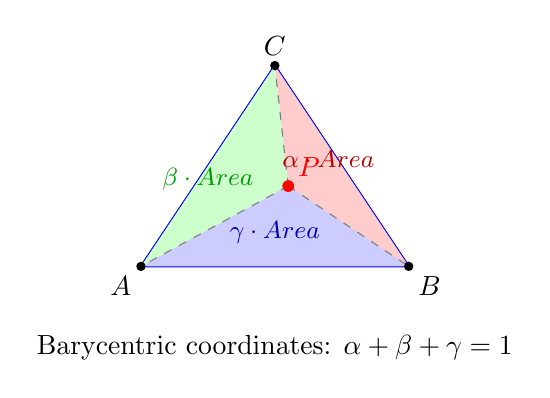
\begin{tikzpicture}[scale=0.85]
    % Source triangle
    \coordinate (A) at (0,0);
    \coordinate (B) at (4,0);
    \coordinate (C) at (2,3);

    % Point P inside
    \coordinate (P) at (2.2,1.2);

    % Draw triangle
    \draw[thick, blue] (A) -- (B) -- (C) -- cycle;

    % Fill sub-triangles with different opacities
    \fill[red!20]   (P) -- (B) -- (C) -- cycle;
    \fill[green!20] (P) -- (C) -- (A) -- cycle;
    \fill[blue!20]  (P) -- (A) -- (B) -- cycle;

    % Draw lines from P to vertices
    \draw[dashed, gray] (P) -- (A);
    \draw[dashed, gray] (P) -- (B);
    \draw[dashed, gray] (P) -- (C);

    % Labels
    \fill[black] (A) circle (2pt) node[below left] {$A$};
    \fill[black] (B) circle (2pt) node[below right] {$B$};
    \fill[black] (C) circle (2pt) node[above] {$C$};
    \fill[red] (P) circle (2.5pt) node[above right] {$P$};

    % Area labels
    \node[red!70!black, font=\small] at (2.8,1.6) {$\alpha \cdot \operatorname{Area}$};
    \node[green!60!black, font=\small] at (1.0,1.3) {$\beta \cdot \operatorname{Area}$};
    \node[blue!70!black, font=\small] at (2.0,0.5) {$\gamma \cdot \operatorname{Area}$};

    \node[below=0.5cm] at (2,-0.3) {Barycentric coordinates: $\alpha+\beta+\gamma=1$};
\end{tikzpicture}
\caption{Barycentric coordinates of point $P$ with respect to triangle $ABC$.  Each coordinate equals the area of the opposite sub-triangle divided by the total area.}
\label{fig:barycentric}
\end{figure}

%-----------------------------------------------------------------------
\subsection{Inverse Mapping vs.~Forward Mapping}
%-----------------------------------------------------------------------

Once we can map the vertices of each triangle, we must decide \emph{how} to transfer pixel values.  There are two fundamentally different approaches.

\paragraph{Forward mapping.}
For each pixel $(x, y)$ in the source image, compute its destination $(x', y') = \mathbf{T}(x, y)$.  This \emph{sounds} natural, but it has a critical flaw: because the transform is not in general integer-preserving, many destination pixels will \emph{never be hit} (they fall between mapped source pixels), producing visible \textbf{holes} in the output.  Rounding to nearest integer mitigates but does not eliminate the problem.

\begin{figure}[htbp]
\centering
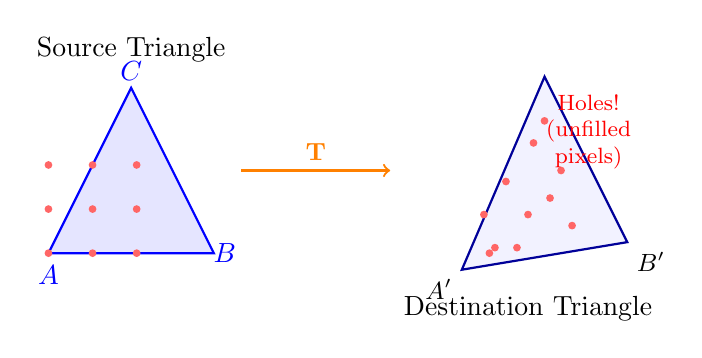
\begin{tikzpicture}[scale=0.7]
    % ---- Source triangle ----
    \begin{scope}[xshift=-5cm]
        \coordinate (A) at (0,0);
        \coordinate (B) at (3,0);
        \coordinate (C) at (1.5,3);

        \draw[thick, blue, fill=blue!10] (A) -- (B) -- (C) -- cycle;

        % Source pixel grid
        \foreach \i in {0,1,2} {
            \foreach \j in {0,1,2} {
                \coordinate (pixel\i\j) at (\i*0.8, \j*0.8);
                \fill[red!60] (pixel\i\j) circle (2pt);
            }
        }

        % Labels
        \node[above] at (1.5,3.3) {Source Triangle};
        \node[blue] at (0,-0.4) {$A$};
        \node[blue] at (3.2,0) {$B$};
        \node[blue] at (1.5,3.3) {$C$};
    \end{scope}

    % Arrow
    \draw[->, thick, orange] (-1.5,1.5) -- (1.2,1.5)
        node[midway, above, font=\small] {$\mathbf{T}$};

    % ---- Destination triangle ----
    \begin{scope}[xshift=2cm]
        \coordinate (A') at (0.5,-0.3);
        \coordinate (B') at (3.5,0.2);
        \coordinate (C') at (2,3.2);

        \draw[thick, blue!60!black, fill=blue!5] (A') -- (B') -- (C') -- cycle;

        % Mapped pixels (sparse, with gaps)
        \fill[red!60] (1.1,0.1)  circle (2pt);
        \fill[red!60] (1.5,0.1)  circle (2pt);
        \fill[red!60] (0.9,0.7)  circle (2pt);
        \fill[red!60] (1.7,0.7)  circle (2pt);
        \fill[red!60] (1.3,1.3)  circle (2pt);
        \fill[red!60] (2.1,1.0)  circle (2pt);
        \fill[red!60] (2.5,0.5)  circle (2pt);
        \fill[red!60] (1.0,0.0)  circle (2pt);
        \fill[red!60] (2.3,1.5)  circle (2pt);
        \fill[red!60] (1.8,2.0)  circle (2pt);
        \fill[red!60] (2.0,2.4)  circle (2pt);

        % Label gaps
        \node[red, font=\footnotesize, align=center] at (2.8,2.2) {Holes!\\(unfilled\\pixels)};

        \node[below] at (1.7,-0.6) {Destination Triangle};
        \node at (A') [below left, font=\small] {$A'$};
        \node at (B') [below right, font=\small] {$B'$};
    \end{scope}
\end{tikzpicture}
\caption{Forward mapping sends discrete source pixels to the destination, leaving gaps (holes).  Not all destination pixels receive a value.}
\label{fig:forward-mapping}
\end{figure}

\paragraph{Inverse mapping.}
Instead of asking ``where does each source pixel go?'', we ask ``where did each destination pixel come from?''.  Concretely, for each pixel $(x', y')$ in the destination, we compute
\[
    \begin{bmatrix} x \\ y \\ 1 \end{bmatrix}
    = \mathbf{T}^{-1}
    \begin{bmatrix} x' \\ y' \\ 1 \end{bmatrix},
\]
where $\mathbf{T}^{-1}$ is the inverse of the affine transform matrix.  We then sample the source image at the (generally non-integer) position $(x, y)$ using interpolation (nearest-neighbor, bilinear, or bicubic).

\paragraph{Why inverse mapping wins.}
\begin{itemize}
    \item \textbf{No holes:} every destination pixel is visited exactly once, so the output is complete.
    \item \textbf{Parallelizable:} each destination pixel can be processed independently.
    \item \textbf{Well-defined:} the only remaining design choice is the interpolation kernel at non-integer source locations.
\end{itemize}

The inverse of a homogeneous affine matrix
\[
    \mathbf{T} =
    \begin{bmatrix}
        \mathbf{A} & \mathbf{t} \\
        \mathbf{0}^\top & 1
    \end{bmatrix}
\]
has the closed form
\[
    \mathbf{T}^{-1} =
    \begin{bmatrix}
        \mathbf{A}^{-1} & -\mathbf{A}^{-1}\mathbf{t} \\
        \mathbf{0}^\top & 1
    \end{bmatrix},
\]
where $\mathbf{A}^{-1} = \frac{1}{\det(\mathbf{A})}
\begin{bmatrix}
    a_{22} & -a_{12} \\
    -a_{21} & a_{11}
\end{bmatrix}$.

\paragraph{Putting it all together.}\label{sec:inverse-mapping}
The complete inverse-mapping warp for a single triangle pair is:
\begin{enumerate}
    \item Compute $\mathbf{T}$ from the three vertex correspondences (Section~2).
    \item Invert $\mathbf{T}$ to obtain $\mathbf{T}^{-1}$.
    \item For each pixel $(x', y')$ in the bounding box of the destination triangle:
    \begin{enumerate}
        \item Compute barycentric coordinates of $(x', y')$ w.r.t.\ the destination triangle.
        \item If any coordinate is negative, the pixel is outside the triangle --- skip it.
        \item Otherwise, apply $\mathbf{T}^{-1}$ to find the corresponding source location $(x, y)$.
        \item Sample the source image at $(x, y)$ by interpolation and write the value to the output.
    \end{enumerate}
\end{enumerate}

This algorithm is fast, exact, and guaranteed to produce a complete output image with no holes.  In the next section we will see how to choose the triangulation that drives all of these individual triangle warps.
